\section{Einleitung}
Der Begriff \textit{Sentiment} stammt vom lateinischen Wort \textit{sentimentum} ab und bedeutet Empfindung oder Stimmung. 
In der Sentimentanalyse geht es um die Bestimmung eben jener Stimmung einer Meinungsäußerung. 
Anwendung findet sie etwa bei Produktbewertungen oder Beiträgen in sozialen Netzwerken. 
Die Stimmung wird durch die sog. Polarität beschrieben und kann positiv, negativ oder neutral ausfallen. 
Im Text-Mining wird sie im Intervall $\interval{-1}{1} = \{x \in \mathbb{R} | -1 \leq x \leq 1\}$ angegeben, wobei -1 sehr negativ, 1 sehr positiv und 0 neutral bedeuten. 

Grundlegend ist die maschinelle Sentimentanalyse entweder Wortlisten- oder Modell-basiert. 
Der Wortlisten-Ansatz kann als eine Sammlung von Worten und ihrer Polaritäten verstanden werden, anhand welcher die Stimmung berechnet wird. 
Dieser Ansatz wird weiter im Kapitel \ref{wortliste} beschrieben, da er in dieser Arbeit verwendet wurde. 

Bei der Modell-basierten Sentimentanalyse wird ein annotierter Satz-Korpus für das Trainieren einer künstlichen Intelligenz vorausgesetzt. 
Etwa für Twitter-Beiträge stehen solche Korpusse oder auch bereits trainierte Modelle zur Verfügung. 
Jedoch ist bei der Verwendung zur Analyse der Sitzungsprotokolle des Bundestages nicht mit zufriedenstellenden Ergebnissen zu rechnen, da sich verwendete Worte und Text- bzw. Satzbau zwischen diesen Domänen deutlich unterscheiden. 
Eine weitere Erläuterung zur Sprache im Bundestag wird in Kapitel \ref{sprachebundestag} gegeben. 

Ebenfalls werden die Komponenten zur Teilnahme an der Verarbeitungspipeline des Gesamtprojektes im nachfolgenden Kapitel \ref{g3daten} beschrieben. 

\section{Datenaustausch}
\label{g3daten}
\subsection{Datenimport}
Für das Erhalten von Daten wurde eine Methode implementiert, welche durch Angabe einer Sitzungs-ID die entsprechende Sitzung vom REST-API von Gruppe 2 abfragen kann. 
Diese Methode gibt jede Sitzung weiter an die in Kapitel \ref{g3textv} beschriebene Textverarbeitung und das Ergebnis schließlich an den in Kapitel \ref{g3export} beschriebenen Export-Code. 

Die Methode wird für zwei Fälle verwendet: 
Beim Normalfall sendet die Gruppe 2 eine Benachrichtigung mit einer Liste aller neuen Sitzungs-IDs an das REST-API im Code dieser Arbeit. 
Das REST-API wurde mit Flask entwickelt und besteht aus einer POST-Schnittstelle, welche auf dem von der HTW bereitgestelltem Server unter \textit{/notify} erreichbar ist. 
Das API wurde unter Zuhilfenahme von \mintinline{latex}{Flask.Blueprints} entwickelt und wird von einem \mintinline{latex}{Waitress}-Webserver bereitgestellt. 
Für jede Anfrage wird geprüft, ob Content-Type und Payload dem erwarteten JSON-Daten entsprechen. 
Sollte dies nicht der Fall sein, wird eine entsprechende Rückmeldung an den Sender zurückgegeben. 
Für jede erhaltene Sitzungs-ID wird die eingangs beschriebene Methode aufgerufen. 

Der zweite Fall wurde vor allem im Rahmen der voranschreitenden Entwicklung bei den in der Projektpipeline voranstehenden Gruppen verwendet. 
Statt auf eine Benachrichtigung zum Anstoßen des Datenimports zu warten, werden stattdessen alle Sitzungs-IDs vom REST-API der Gruppe 2 abgefragt und jede Sitzung vollständig neu importiert. 
Dieses Vorgehen hat den Vorteil, dass eventuell durch Arbeit am Code verpasste Benachrichtigungen nachgeholt werden und gleichzeitig Änderungen an den Daten übernommen werden können. 

\subsection{Datenexport}
\label{g3export}
Statt Arbeit in ein umfangreiches REST-API für die nachfolgenden Gruppen zu stecken, wurde für diese Arbeit ein reiner MongoDB-Ansatz verwendet. 
Auf dem zur Verfügung stehenden HTW-Server wurde dafür eine MongoDB Instanz aufgesetzt, welche nur aus dem HTW-Netz erreichbar und zudem nur mit Authentifizierung zugreifbar ist. 
Jede Sitzung ist hier als eine eigene Collection persistiert. 
Sobald neue Sitzungen importiert und verarbeitet wurden, werden diese zunächst mit dem MongoDB-Treiber \mintinline{latex}{PyMongo} in die Datenbank geschrieben. 
Anschließend werden die nachfolgenden Gruppen mit einem POST and die jeweilige REST-Schnittstelle benachrichtigt, dass neue Daten vorliegen. 
Diese greifen dann mit den zuvor versendeten Zugangsdaten direkt auf die Datenbank zu. 
Mit diesem Vorgehen konnte die Komplexität beim Zugriff auf die Ergebnis-Daten gesenkt werden, da es für nahezu alle gängigen Programmiersprachen einen intuitiven MongoDB-Treiber gibt. 

\section{Wortliste}
\label{wortliste}
Wie bereits in der Einleitung beschrieben, handelt es sich bei Wortlisten in der Sentimentanalyse um eine Liste von Worten und ihrer jeweiligen Polarität. 
Bei der Analyse eines Textes wird wortweise ein Abgleich mit dieser Liste durchgeführt und die Wort-Polarität bei einer Übereinstimmung für die Berechnung des Sentiments verwendet. 
Unterschiedliche Berechnungsformeln sind dabei denkbar und werden in Kapitel \ref{polberechnung} weiter besprochen. 
Für diese Arbeit wurden Wortlisten verschiedener Institutionen kombiniert und anschließend mit Synonymen erweitert. 
Ebenfalls wurde eine eigene Bundestags-Wortliste erstellt. 

Die Interest Group on German Sentiment Analysis (IGGSA) stellt eine umfangreiche Liste an Publikationen und Ressourcen zu Sentimentanalysen in der deutschen Sprache zur Verfügung. 
Hier wurden alle Referenzen auf die in dieser Arbeit verwendeten Quell-Wortlisten gesammelt. 
Für die Zusammenführung dieser Wortlisten wurden zunächst zwei Herangehensweisen evaluiert: 
Zum einen war die Erstellung eines eigenständigen Codes denkbar, welcher einmalig die Daten aus allen Quellen einliest, zusammenfasst und eine Ergebnis-Datei ausgibt. 
Diese Datei wäre eine Ressource für den eigentlichen Analyse-Code. 
Zum anderen könnte die soeben beschriebene Funktionalität jedoch auch direkt im Analyse-Code integriert und bei jedem Programmstart ausgeführt werden. 
Die kombinierte Wortliste würde somit nicht auf die Festplatte geschrieben, sondern im Arbeitsspeicher verbleiben, solange der Analyse-Code läuft. 
Wenngleich der zuerst beschriebene Ansatz offensichtlich weniger Rechenzeitaufwändig ist, wurde für diese Arbeit der zweite Ansatz gewählt. 
Dies wird vor allem mit Rechtsunsicherheiten bei der Arbeit mit den verschiedenen Lizenzen der Quelldateien begründet. 
Gleichzeitig arbeitet der Analyse-Code damit jederzeit mit dem aktuellen Stand der Quell-Wortlisten. 
Das Aufbauen der Wortliste dauert wenige Minuten. 

Für diese Arbeit wurden die folgenden Quell-Wortlisten verwendet: 

\begin{itemize}
\item \textit{SentimentWortschatz} (SentiWS) aus "SentiWS - a Publicly Available German-language Resource for Sentiment Analysis" (Universität Leipzig)
\item \textit{German Polarity Lexicon} aus "Evaluation and extension of a polarity lexicon for German" (Universität Zürich)
\item \textit{morphcomp} aus "Evaluating the morphological compositionality of polarity" (Leibniz-Institut für Deutsche Sprache, Universität des Saarlandes)
\end{itemize}

Aus diesen Quellen ergibt sich eine Wortliste mit etwa 14.000 einzigartigen Worten. 
Die Worte werden dabei mit der in Kapitel \ref{g3textv} beschriebenen Textverarbeitungspipeline lemmatisiert, also auf die Grundform zurückgeführt. 
Bei Überschneidungen wird ein Mittelwert über alle Polaritäts-Werte eines Wortes gebildet. 

Mithilfe des \textit{Open German WordNet} (OdeNet) werden zu jedem Wort Synonyme gesammelt und ebenfalls der Wortliste hinzugefügt. 
Der Zugriff auf OdeNet geschieht dabei mit der python Bibliothek \mintinline{latex}{WN}. 
Die Verwendung dieser Bibliothek ist trivial, weshalb an dieser Stelle keine weitere Erläuterung gegeben wird. 
Die Wortliste wird durch das Hinzufügen von Synonymen um weitere rund 2.000 Worte erweitert. 

Wie bereits in der Einleitung erwähnt, wurde zudem eine eigene Bundestags-Wortliste erstellt. 
Hierzu wurden die 15.000 am häufigsten in den Sitzungsprotokollen vorkommenden Worte erfasst und analysiert. 
Dabei wurden jedoch nur jene Worte betrachtet, welche nicht bereits in der kombinierten Wortliste vorkommen. 
Ausgewählt wurden nur eindeutig positive oder negative Worte wie \textit{angemessen}, \textit{Bullshit}, \textit{Fehlentscheidung}, \textit{Milchmädchenrechnung}, \textit{Realitätsverweigerung}, \textit{Totalausfall} oder \textit{Verunglimpfung}. 
Insgesamt umfasst die Bundestags-Wortliste 217 Worte. 

Im Code wird der Zugriff auf die Wortliste mit der zentralen Klasse \mintinline{latex}{Lexicon} realisiert. 
Bei der Instanziierung der Klasse werden, wie im Vorherigen beschrieben, alle Wortlisten gesammelt, zusammengeführt und erweitert. 
Anschließend stellt die Klasse ein \mintinline{latex}{Dictionary} bereit, in welchem die Schlüssel die Worte und die Werte die Wort-Polarität angeben. 

\section{Textverarbeitung}
\label{g3textv}
Für die Textverarbeitung nutzt der Code dieser Arbeit vollständig die Funktionalitäten und Strukturen von \mintinline{latex}{spaCy}. 
Die \mintinline{latex}{spaCy} Bibliothek stellt eine Textverarbeitungspipeline bereit, welche mithilfe eines vortrainierten Modells funktioniert. 
Für die deutsche Sprache wurde ein solches Modell mit dem TIGER Korpus der Universität Stuttgart trainiert. 
Der Korpus umfasst ca. 50.000 Sätze aus Texten der Frankfurter Rundschau. 
Die \mintinline{latex}{spaCy}-Pipeline besteht aus den folgenden Komponenten: 

\begin{itemize}
\item Tokenisierung (Text- und Satzzerteilung)
\item POS-Tagging (Wortartenerkennung)
\item Dependency-Parsing (Wortabhängigkeitenerkennung)
\item Lemmatisierung (Wortgrundformermittlung)
\item Entity-Recognition (Eigennamenerkennung)
\end{itemize}

Das Ergebnis der Pipeline ist ein \mintinline{latex}{Doc}-Objekt, welches das Ergebnis des gesamten in die Pipeline gegebenen Textes umfasst. 
Einzelne Sätze innerhalb des \mintinline{latex}{Doc}-Objektes werden mit \mintinline{latex}{Span}-Objekten beschrieben und einzelne Worte mit \mintinline{latex}{Token}-Objekten. 
Die Objekttypen besitzen jeweils eigene Methoden und Erweiterungsmöglichkeiten in Form von sog. \textit{extension attributes}. 

Sehr einfach und gleichzeitig umfangreich kann die \mintinline{latex}{spaCy}-Pipeline an die eigenen Bedürfnisse angepasst werden. 
So wurde die Berechnung des Sentiments eines Textes direkt an die Komponenten der Standart-Pipeline angehängt. 
Logisch unterteilt sich diese in die Komponenten:

\begin{itemize}
\item Negations-Erkennung (siehe \ref{neg-erkennung})
\item Verstärkungs-Erkennung (siehe \ref{ver-erkennung})
\item Polaritätsberechnung (siehe \ref{polberechnung})
\end{itemize}

Basis für das nachfolgende Kapitel \ref{neg-erkennung} ist dabei das Ergebnis des Dependency-Parsers von \mintinline{latex}{spaCy}. 
Dieser bestimmt die Abhängigkeiten zwischen den einzelnen Elementen eines Satzes. 
Diese Funktion gehört dem Themenbereich der Dependenzgrammatik an, in welcher gerichtete Beziehungen zwischen den Worten eines Satzes beschreibt werden. 
Ein Wort kann einen Vorgänger (Regent) und mehrere Nachfolger (Dependenten) besitzen. 
Die Gesamtheit der Beziehungen eines Satzes wird auch Abhängigkeitsbaum genannt. 

Zur Verdeutlichung soll die Abbildung \ref{steffi} dienen, welche mithilfe von \mintinline{latex}{spaCy.displaCy} erstellt wurde. 
Zu sehen ist hier der Abhängigkeitsbaum des Satzes \textit{\glqq Das ist doch fachlich Quatsch hoch sechs!\grqq}. 
An den gerichteten Kanten befindet sich die Angabe des Satzgliedes, unterhalb der Worte die Angabe der Wortart. 

\begin{figure}[htb]
\centerline{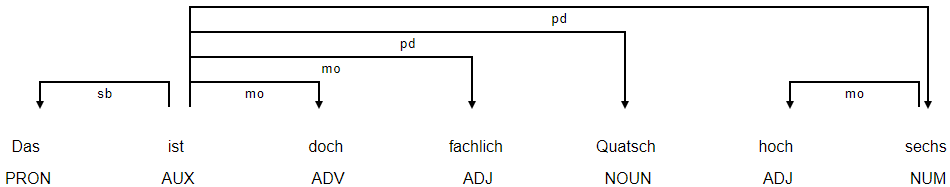
\includegraphics[width=1\textwidth]{steffi.png}}
\caption{Visualisierung der Wortabhängigkeiten (Zitat von Steffi Lemke MdB, 208. Sitzung, 10.02.2021)}
\label{steffi}
\end{figure}

\subsection{Negations-Erkennung}
\label{neg-erkennung}
Negation, also Ablehnung, Verneinung oder Aufhebung, hat einen erheblichen Einfluss auf das Ergebnis und damit die Korrektheit der Sentimentanalyse, weshalb in dieser Arbeit ein besonderes Augenmerk auf ihre Erkennung gelegt wurde. 
In \textit{Negation Modeling for German Polarity Classification} präsentieren Forscher der Universität des Saarlandes und des Leibniz-Institut für Deutsche Sprache hierfür einen regelbasierten Ansatz. 

Sie definieren unterschiedliche Negationstypen und ihre jeweilige Reichweite. 
So beeinflussen etwa negierende Adverbien oder Indefinitpronomen wie \textit{nie} den gesamten Satz, wohingegen das Partikel \textit{nicht} lediglich seinen Vorgänger negiert.  
Die Tabelle \ref{tab1} führt alle in dieser Arbeit implementierten Negationsregeln auf. 
Die Nutzung eines Abhängigkeitsbaumes, wie von \mintinline{latex}{spaCy} ermittelt, ist dabei unerlässlich. 
Denn wie schon im vorherigen Kapitel angesprochen, ist etwa mit dem Vorgänger eines Wortes nicht das in der Satzabfolge voranstehende Wort gemeint, sondern vielmehr der semantische Regent. 

\begin{table}[htbp]
\caption{Implementierte Negations-Regeln aus X}
\begin{center}
\begin{tabular}{| c | c | c |}
\hline
Negationstyp & Reichweite & Beispielworte \\ \hline
Partikel & Vorgänger (Regent) & nicht \\ \hline
Präpositionen & Nachfolger (Dependent) & ohne, gegen \\ \hline
Adverbien, Indefinitpronomen & Satz & nie, kein, kaum \\ \hline
Nomen & Genitiv, Präpositionalobjekt & Abschaffung, Zerstörung \\ \hline
Verben & Objekt, Subjekt & enden, sinken, lindern \\
\hline
\end{tabular}
\label{tab1}
\end{center}
\end{table}

Angemerkt sei an dieser Stelle, dass es nicht möglich war, alle Regeln aus X zu implementieren, da der von den Forschern genutzte Dependency-Parser umfangreichere Ergebnisse liefert, als jener von \mintinline{latex}{spaCy}. 

Eine Liste mit Negationsworten und dem jeweiligen Negationstyp wurde X entnommen und ist ebenfalls über die Klasse \mintinline{latex}{Lexicon} zugreifbar. 
Die Klasse stellt ein \mintinline{latex}{Dictionary} bereit, in welchem die Schlüssel die Negationsworte und die Werte eine Liste der Reichweiten sind. 

Wenn in einem Text ein Negationswort auftritt, werden alle implementierten Regeln geprüft. 
Sollte es zu einem Treffer kommen, etwa wenn das Wort \textit{nicht} auftritt (siehe Abb. \ref{brandner}) und es einen Vorgänger gibt, werden alle Worte in Reichweite des Negationswortes negiert. 
Dies geschieht, indem für die jeweiligen Worte, welche wie in \ref{g3textv} beschrieben \mintinline{latex}{Token}-Objekte sind, ein eigenes Attribut mit der Bezeichnung \mintinline{latex}{negated} auf \mintinline{latex}{True} gesetzt wird. 
In der Polaritätsberechnung wird wortweise auf dieses Attribut geprüft und die Wort-Polarität bei einer Negierung mit -1 multipliziert. 

\begin{figure}[htb]
\centerline{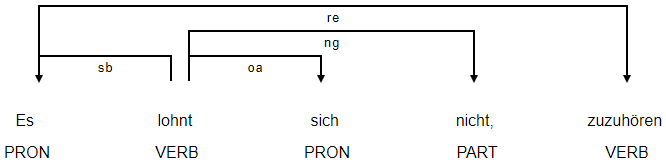
\includegraphics[width=1\textwidth]{brandner.png}}
\caption{Beispielsatz mit Patikel-Negation (Zitat von Stephan Brandner MdB, 207. Sitzung, 29.01.2021)}
\label{brandner}
\end{figure}

\subsection{Verstärkungs-Erkennung}
\label{ver-erkennung}
Als \textit{Verstärker} werden sog. Gradpartikel (z.B. sehr, besonders, viel) verstanden, welche direkt vor Adjektiven oder Adverbien in einem Satz auftreten. 
Sie verstärken ihren Nachfolger, was wiederum in der Polaritätsberechnung berücksichtigt werden soll. 

Aus diesem Grund wird eine Liste mit verstärkenden Gradpartikeln, welche aus der gleichen Quelle wie in Kapitel \ref{neg-erkennung} bezogen werden, eingelesen und über die \mintinline{latex}{Lexicon} Klasse bereitgestellt. 

Ebenso wie in Kapitel \ref{neg-erkennung} bereits für die Negation beschrieben, wird ein eigenes Attribut zur Signalisierung einer Verstärkung definiert und im entsprechenden Fall auf True gesetzt. 
Bei der Polaritätsberechnung wird bei einer erkannten Verstärkung die Wort-Polarität mit 1,5 multipliziert. 

In Abbildung \ref{hessel} wird ein Beispiel für das Auftreten eines verstärkenden Gradpartikels gegeben. 
Hier verstärkt das Wort \textit{sehr} das negative Wort \textit{spät}, womit die errechnete Polarität stärker negativ ausfällt als ohne die Verstärkungs-Erkennung. 

\begin{figure}[htb]
\centerline{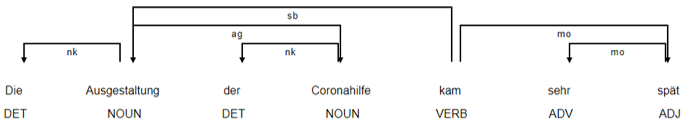
\includegraphics[width=1\textwidth]{hessel.png}}
\caption{Beispielsatz mit Gradpartikel-Verstärkung (Zitat von Katja Hessel MdB, 206. Sitzung, 28.01.2021)}
\label{hessel}
\end{figure}

\subsection{Polaritätsberechnung}
\label{polberechnung}
Für die abschließende Berechnung der Polarität sind verschiedene Formeln denkbar. 
Sie sollten anhand von Textcharakteristika wie z.B. der Satz- oder Textlänge gewählt werden. 

Bei der Verwendung einer satzbasierten Polaritätsberechnung, bei welcher alle Polaritäten erst addiert und die Summe anschließend durch die Anzahl der Worte dividiert wird, kann ein unerwünschtes Phänomen auftreten: 
Längere Sätze erhaltenen ein stärker polarisiertes Ergebnis als vergleichbare kurze Sätze. 

Dies ist mit einer im Schnitt höheren Dichte an Worten mit Polaritäts-Wert in längeren Sätzen zu erklären. 
Aus diesem Grund wurde in dieser Arbeit eine Min-Max-Skalierung (siehe Formeln 1 - 3) auf Dokumentebene implementiert. 

Die Entscheidung, diese Normalisierung anhand der Länge des gesamten Textes durchzuführen, wurde aufgrund der Charakteristika der zu analysierenden Interaktionen getroffen. 
Denn diese bestehen zu einem überwiegenden Teil aus einem einzelnen Satz von jedoch sehr unterschiedlicher Länge. 

\begin{align}
p' &= \frac{ p + 1 }{ text.len + 1 } \text{ für p $>$ 0}\\
p' &= \frac{ p - 1 }{ text.len + 1 } \text{ für p $<$ 0}\\
p' &= p \text{ für p $=$ 0}
\end{align}

\section{Evaluierung}
\subsection{Sprache im Bundestag}
\label{sprachebundestag}
Während der Entwicklung dieser Arbeit und den regelmäßig angestellten Zwischentests wurde ersichtlich, dass sich die Sprache im Bundestag etwa von jener in sozialen Netzwerken oder Produktbewertungen unterschiedet. 
Ein Interaktionstext setzt sich sowohl aus einzelnen, langen und komplexe Sätze zusammen, als auch aus einzelnen Ausrufen wie \textit{\glqq eieiei!\grqq} zusammen. 

Aus diesem Grund wurde die in \ref{polberechnung} beschriebene Normalisierung verwendet, da herkömmliche Berechnungsformeln zunächst widersprüchliche Ergebnisse lieferten. 
Gleichzeitig verbesserte die manuelle Durchsicht der häufigsten 15.000 Worte und Anfertigung einer eigenen Bundestags-Wortliste das Ergebnis deutlich. 
Viele der regelmäßig in Bundestagssitzungen verwendeten Worte gehören zur \textit{Politik-Domäne} und treten deshalb nicht in den Quell-Wortlisten auf. 
Hier wird erwartet, dass eine noch umfangreichere Bundestags-Wortliste einen weiteren positiven Einfluss auf das Endergebnis hätte. 
Aus Zeit- sowie Kompetenzgründen wurde diese Liste jedoch nicht erweitert. 

\subsection{Ironie und Sarkasmus}
Ebenso wie die im vorherigen besprochene \textit{Politiksprache}, treten auch Ironie und Sarkasmus vermehrt in den Sitzungen des Bundestages auf. 
Einfach umrissen, handelt es sich dabei um ein Stilmittel, bei dem das Gegenteil vom Gesagten gemeint ist. 
Sarkasmus ist dabei eine verstärkte Form der Ironie und kann auch als ein Angriff verstanden werden. 

Selbst für den menschlichen Leser ist allein am geschriebenen Text nicht immer ersichtlich, ob eine Aussage ironisch gemeint ist. 
Vielmehr wird für die richtige Deutung die Stimmlage, Gestik und Mimik der sprechenden Person benötigt. 

Ironie und Sarkasmus könne also erst recht nicht mit dem in dieser Arbeit verwendeten Wortlisten-Ansatz erkannt werden, womit ein unbekannter Teil der Interaktionen im Ergebnis die falsche Polarität besitzt. 
Gleichwohl gibt es Ansätze aus dem Bereich des maschinellen Lernens, welche dieses Problem behandeln. 
Jedoch setzen diese einen entsprechend annotierten Korpus vorraus und stammen zudem aus dem Bereich der sozialen Netzwerke, in welchen etwa mit \textit{Hashtags} die Ironie bereits vom Autor markiert wurde. 

\subsection{Fazit}
Trotzt der soeben beschriebenen Fehlerquellen, wurde dennoch ein gelungenes Ergebnis erzielt: 
Es wurde ein solider und erweiterbarer Algorithmus zur Sentimentananlyse von Texten geschaffen, welcher auf den bekanntesten Bibliotheken und Techniken der Textverarbeitung beruht. 
Dieser kann als Basis für weitere Anstrengungen bei der Sentimentanalyse von politischen Texten dienen. 

Eine Deutung der bisherigen Ergebnisse durch Politikwissenschaftler oder anderweitig in diesem Bereich kompetente Personen wird dabei empfohlen, um die beschriebenen Schwachstellen entsprechend zu behandeln oder neue zu identifizieren. 

Der Programmcode ist zudem vollständig und abgesichert in die Projektpipeline eingebunden. 
Er erweitert seine Ergebnis-Datenbank automatisch um neue Sitzungen und benachrichtigt anschließend nachfolgende Gruppen. 
